\section{Sequenzdiagramme Web}

%Im Folgendem sind Sequenzdiagramme für elementare Anwendungsfälle gegeben. Sie sollen einen Eindruck bieten, wie für diese die Kommunikation 

\begin{figure}[H]
	\centering
	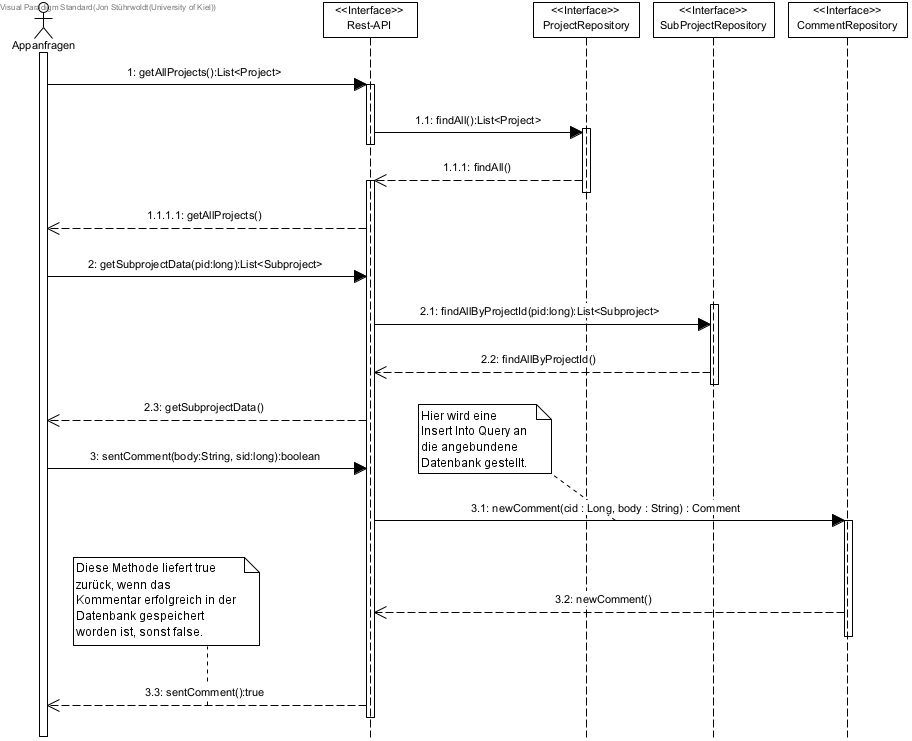
\includegraphics[width=\textwidth]{img/seqwebcreate}		
	\caption{Sequenzdiagramm - Kommentar schreiben}
	\label{fig:sequenz-a}
\end{figure}

Dieses Sequenzdiagramm zeigt den zeitlichen Ablauf des Anwendungsfalles "Kommentar bei Teilprojekt abgeben". Die App fragt hierbei beim Backend
zuerst die Projektdaten, dann die Teilprojektdaten und schließlich die jeweiligen Kommentarlisten der Teilprojekte an. Die einzelnen Anfragen werden
dabei über eine Rest-API geregelt, welches dann im Backend die zur Anfrage gehörigen Daten aus den Repositories abfragt und anschließend wieder an die
App zurücksendet.


\begin{figure}[H]
	\centering
	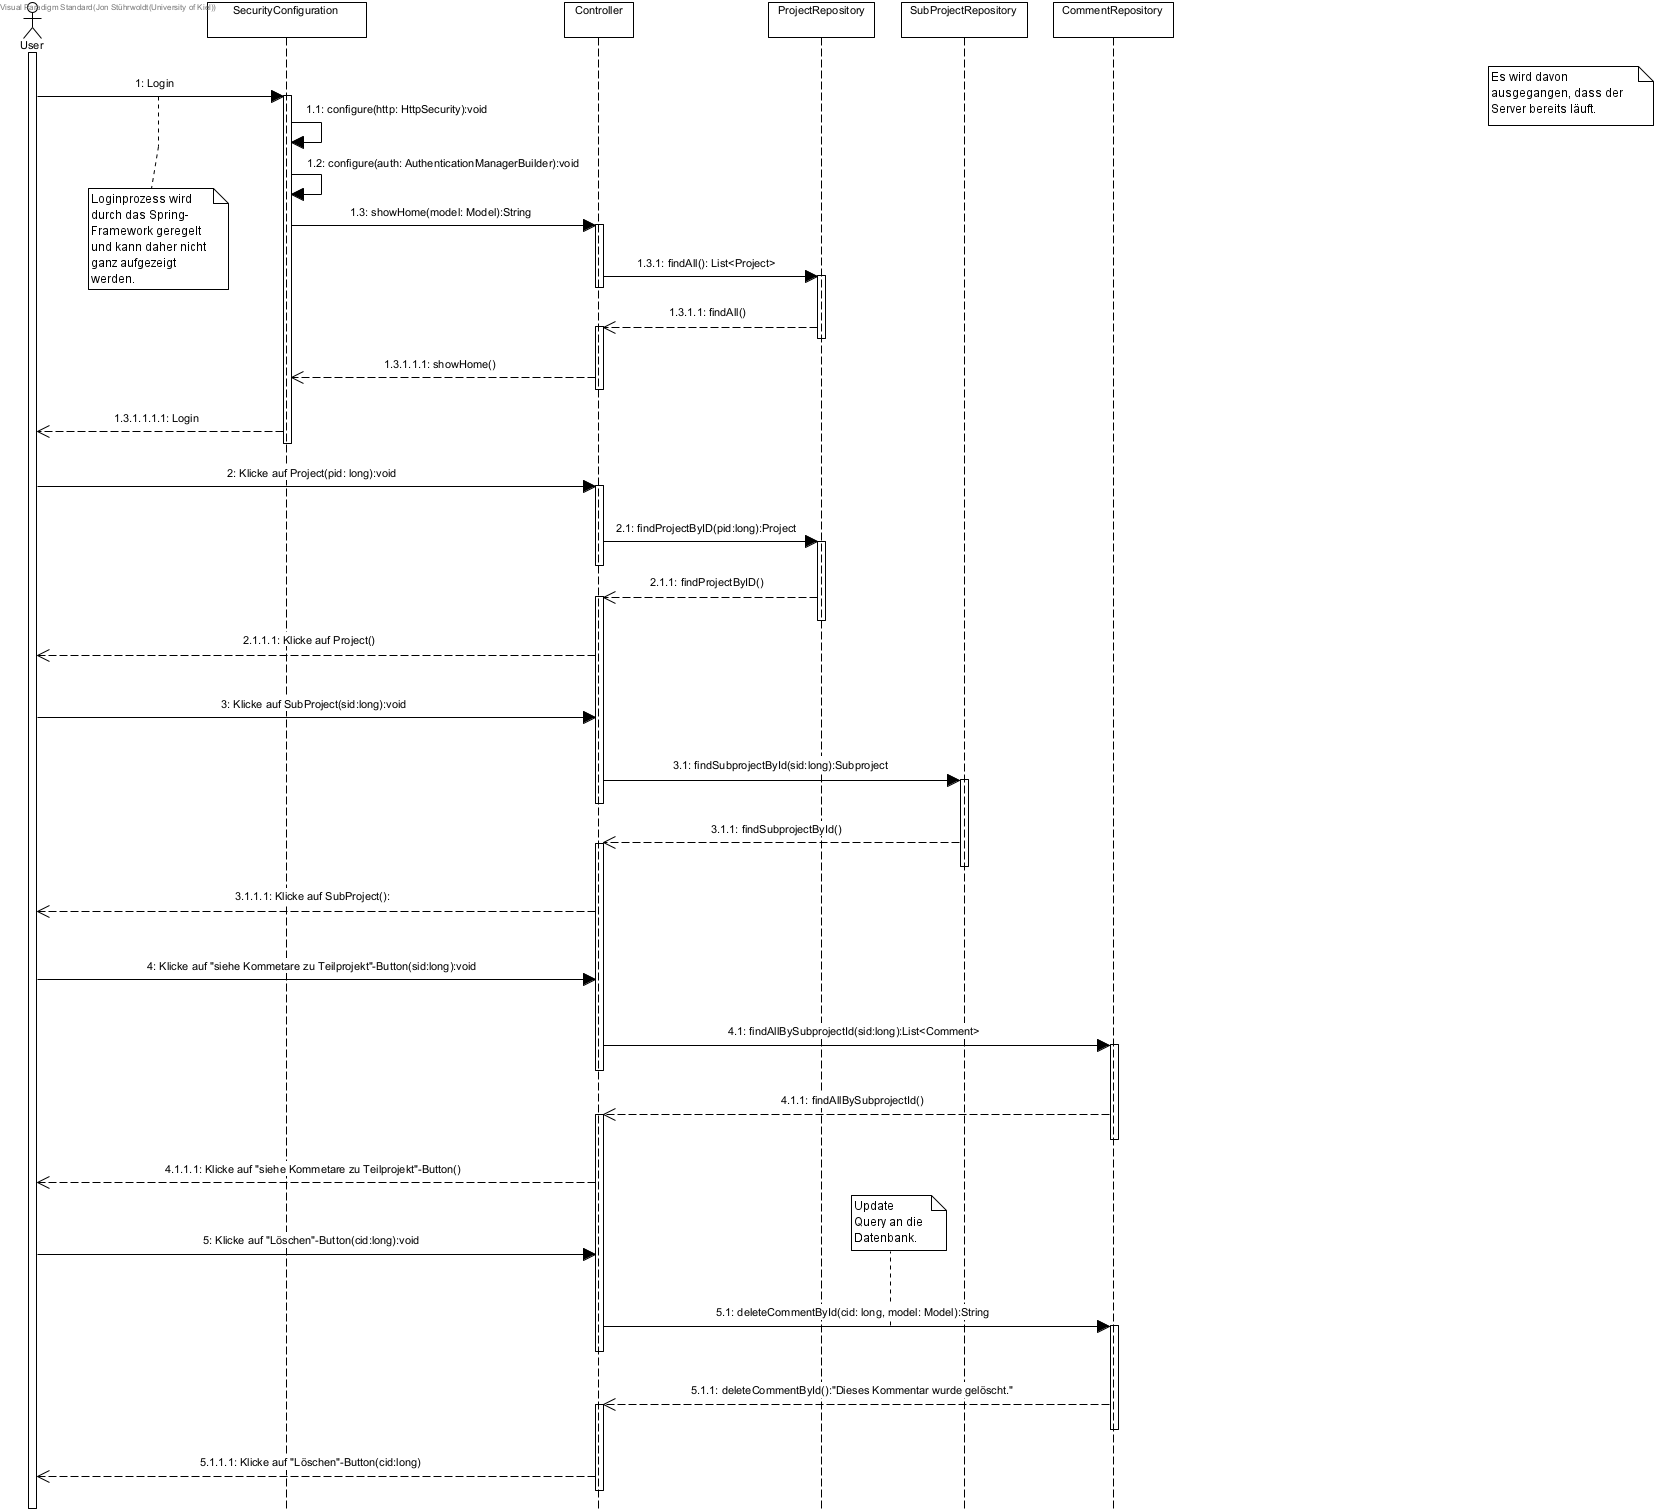
\includegraphics[width=\paperwidth]{img/seqwebdelete}		
	\caption{Sequenzdiagramm - Kommentar löschen}
	\label{fig:sequenz-b}
\end{figure}

Dieses Sequenzdiagramm zeigt den zeitlichen Ablauf des Anwendungsfalles "Kommentar löschen". Um die Berechtigung zu haben, Kommentare löschen zu
können, muss sich der User als Admin einloggen. Der Login-Prozess wird vom Spring Boot Framework übernommen. Nach einem erfolgreichen Login wird
man dann zur ``Home``-Seite weitergeleitet. Dabei wird die Methode showHome() vom Controller aufgerufen, der sich erst die nötigen Daten aus dem
jeweiligen Repository zieht und anschließend eine auf den Daten basierende .html Datei zurückgibt. Der Ablauf vom Controller bis zur .html Datei
geschieht analog mit den Daten vom Projekt, Teilprojekt und Kommentar. 


\section{Sequenzdiagramme App}


\begin{figure}[H]
	\centering
	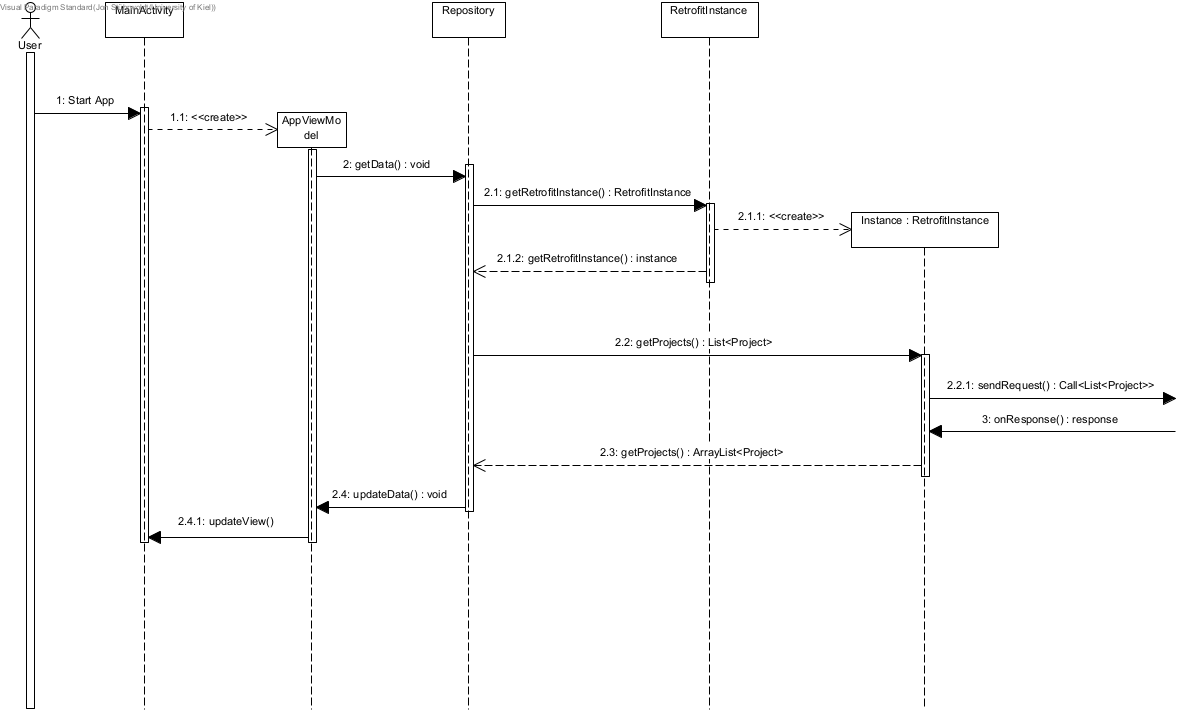
\includegraphics[width=\textwidth]{img/seqappstart}		
	\caption{Sequenzdiagramm - App starten}
	\label{fig:sequenz-c}
\end{figure}

Dieses Sequenz-Diagramm beschreibt den App-Aufruf und das Afragen der Projektdaten über das Backend. Nach dem Start der App initialisiert die MainActivity das AppViewModel. Das AppViewModel stellt eine Anfrage an das Repository. Dort wird eine RetrofitInstance erstellt, über welche die Projektdaten vom Backend abgefragt werden. Die Daten werden zum AppViewModel zurückgegeben und auf der MainActivity dargestellt.


\begin{figure}[H]
	\centering
	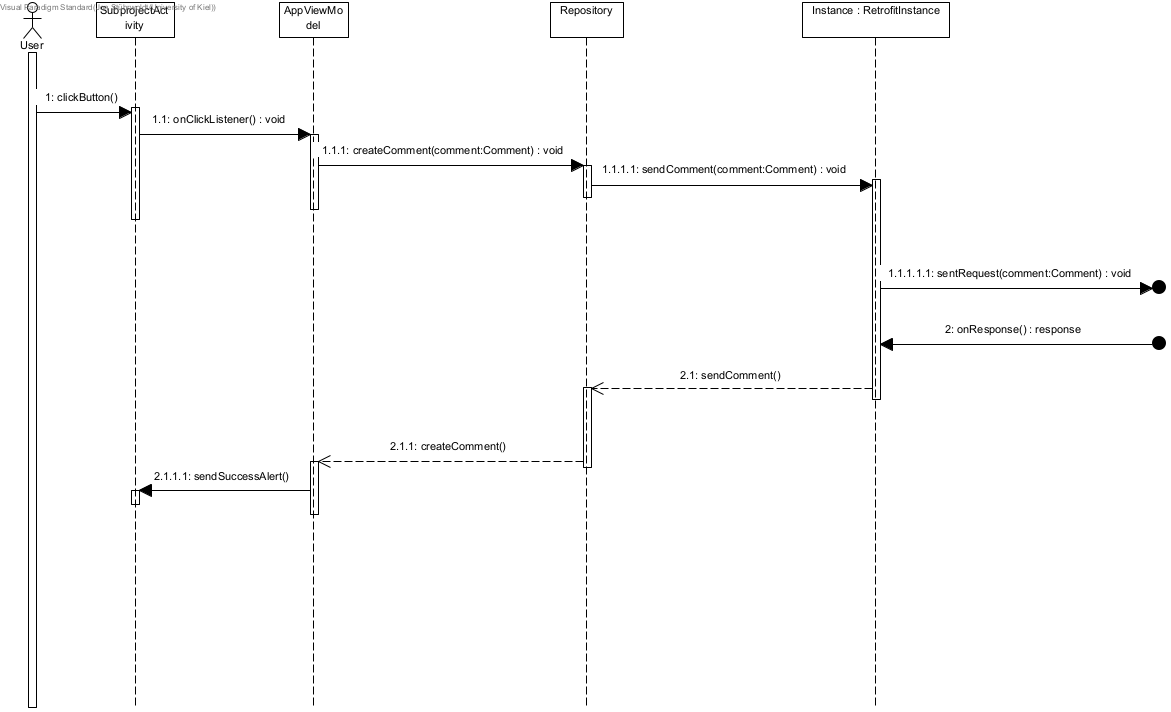
\includegraphics[width=\textwidth]{img/seqappcreate}		
	\caption{Sequenzdiagramm - Kommentar schreiben}
	\label{fig:sequenz-d}
\end{figure}

Die Abbildung zeigt das Sequenz-Diagramm zum Hinzufügen eines neuen Kommentars zu einem Teilprojekt. Nach dem Eingeben des Kommentars kann er über einen Button die Eingabe bestätigen. Dabei ruft das AppViewModel eine Methode zum Erstellen eines neuen Kommentars im Repository auf. Das Repository leitet den Kommentar weiter an das Backend. Im Anschluss wird eine Success-Message an den Benutzer zurückgegeben. 